
\ifdraft{\color{red}}{}\chapter{Desenvolvimento da Aplicação}

Essencialmente a aplicação foi desenvolvida em linguagens Web, o JavaScript sendo a linguagem de programação, HTML como linguagem de marcação e CSS como estilização. Nesse modelo já existem editores de código fonte de linguagens de programação,dos mais utilizados temos ACE e o CodeMirror, optado pelo primeiro pois em análise entendeu-se como sendo mais prático para o uso e criação do modelo da linguagem. Considerou-se a criação do modelo gramatical para destaque da sintaxe como dificuldade relativamente baixa.

Para resultar na árvore gramatical encontrou-se o ACORN um parser já escrito em JavaScript. De modo trabalhoso foi necessário adaptar o código fonte para compreender a estrutura do algorítmos proposto, principalmente devido à não utilização de parênteses para o comando de impressão em tela na linguagem UAL.

Como saída o interpretada o JS-Interpreter foi encontrado como a única opção. Ele já se utiliza do mesmo ACORN mencionado acima e interpreta a própria linguagem JavaScript. Pelo mesmo motivo citado acima, falta de parênteses no comando, se tornou uma tarefa um tanto dispendiosa fazer com que ele se adaptasse ao modelo.

\begin{figure}[h]
  \caption{Interface Desktop}\label{fig:ui-pc}
  \centering
  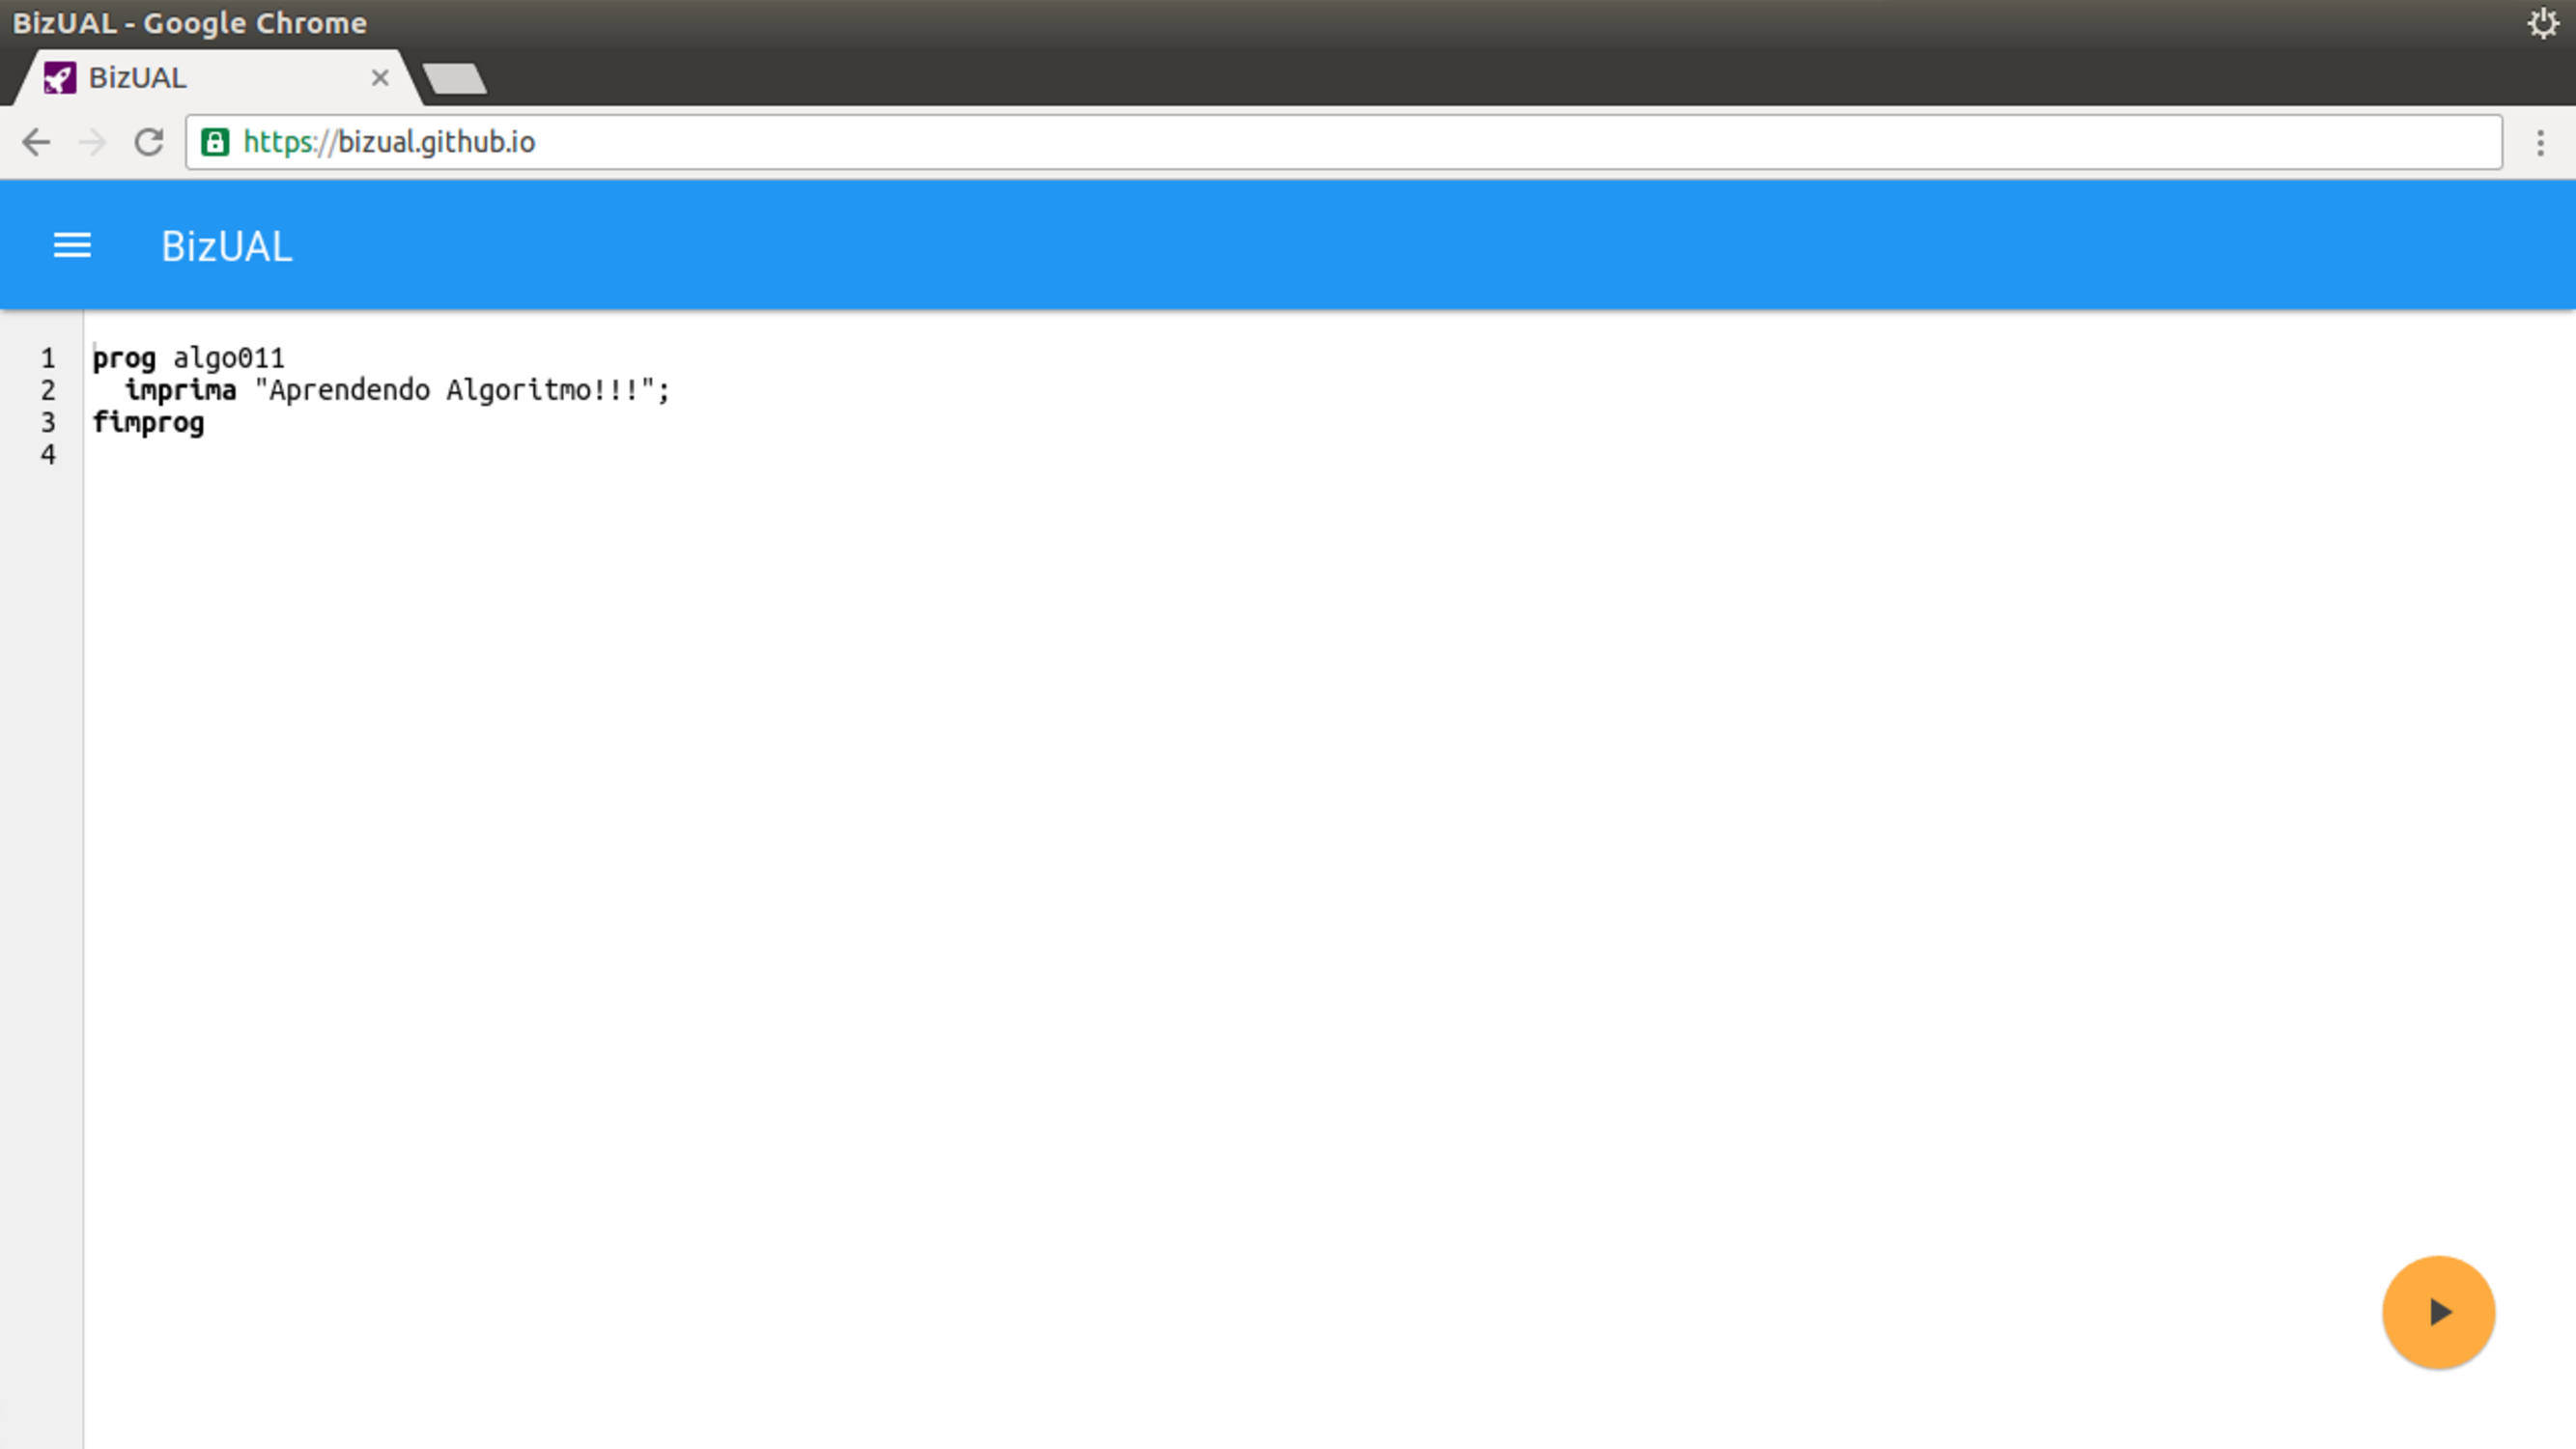
\includegraphics[width=10cm,height=10cm,keepaspectratio]{figures/bizual-desktop.pdf}
  \caption*{\footnotesize Fonte: Autor}
\end{figure}

Como interface gráfica foi mantido o mínimo necessário. Somente o editor de texto e um botão para executar. Foram visualizadas renderizações e tamanhos de telas variados, computadores (Figura \ref{fig:ui-pc}), tablets, smartphones (Figura \ref{fig:ui-phone}), etc. Seguindo conceitos do Google Material Design foi adicionada uma barra no topo como botão para menu o nome da aplicação, denominada Bizu, e um botão flutuante no canto inferior direito como ícone ``play'' para a execução do algoritmo.

\begin{figure}[h]
  \caption{Interface Smartphone}\label{fig:ui-phone}
  \centering
  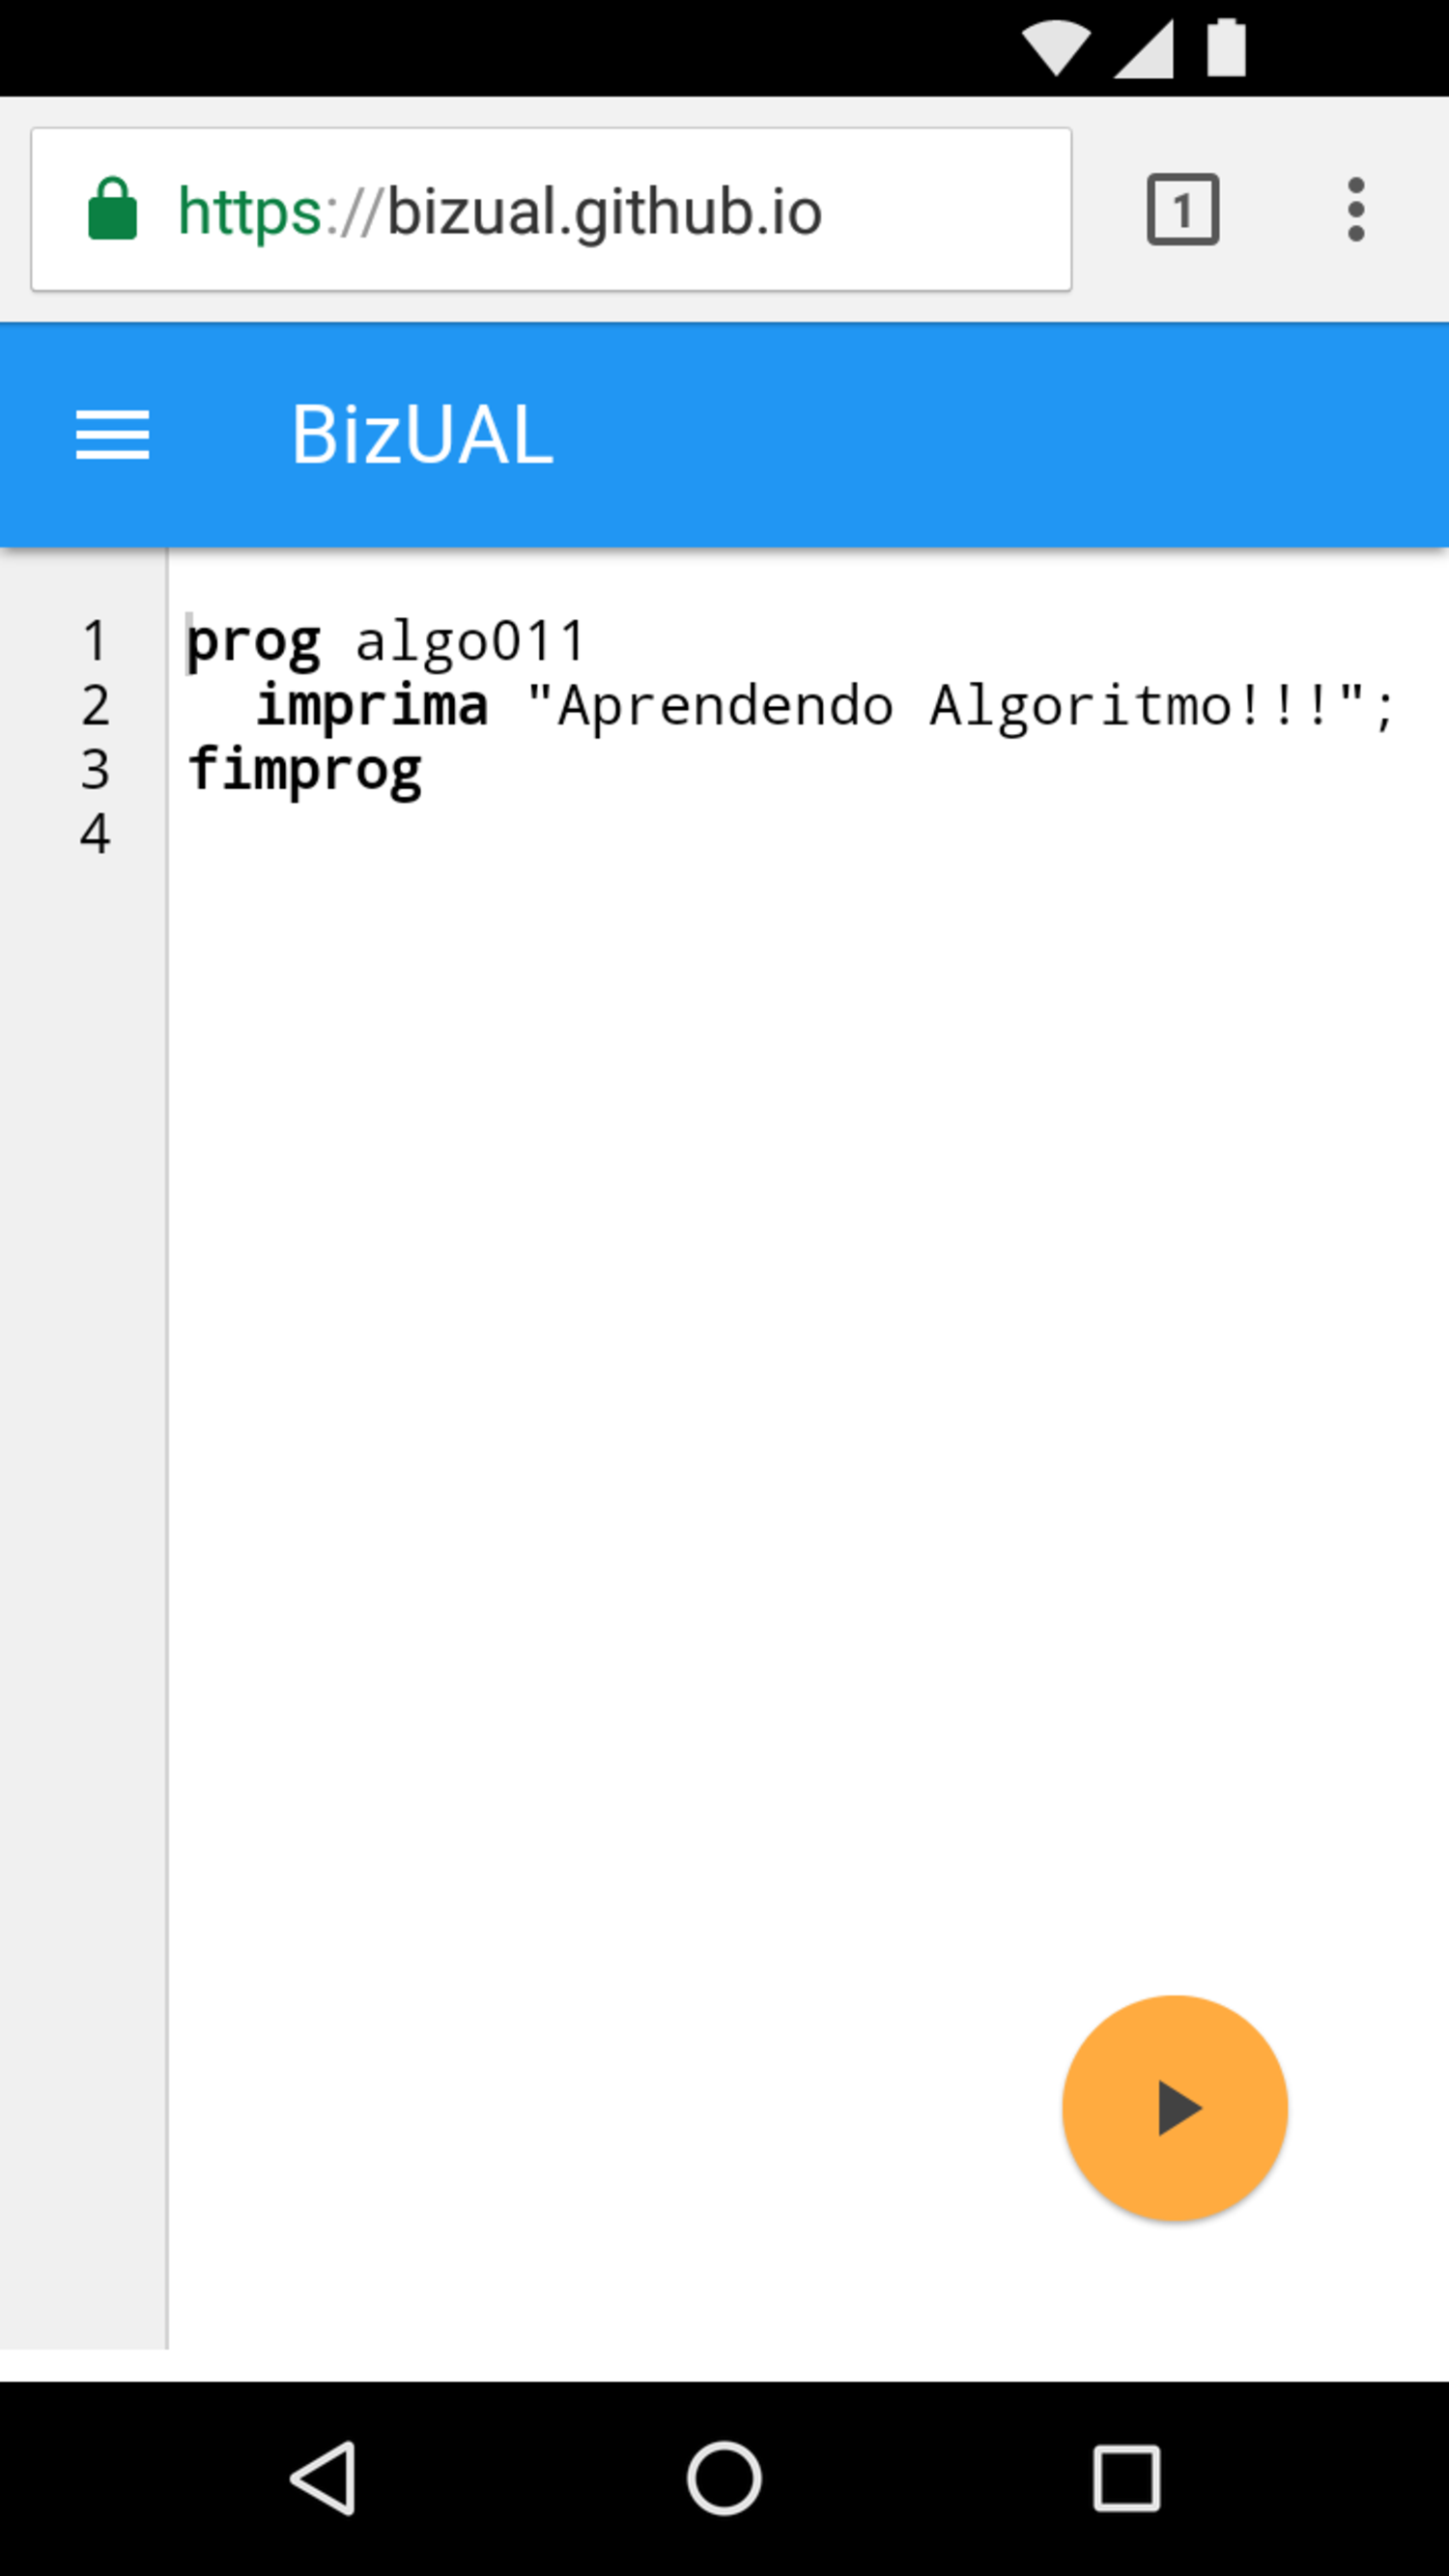
\includegraphics[width=10cm,height=10cm,keepaspectratio]{figures/bizual-smartphone.pdf}
  \caption*{\footnotesize Fonte: Autor}
\end{figure}

Facilitando a tarefa de construção da interface foi utilizada a biblioteca Material Design Lite (MDL) disponibilizada oficialmente pelo Google. As cores foram escolhidas pela funcionalidade disponível no site da biblioteca.
A escolha do nome se deve a partir da palavra bizu adicionada a sigla da sintaxe.
Foi utilizado a funcionalidade app cache a partir de um arquivo manifesto listando o conteúdo que o navegador deve guardar cópia local. Podendo assim ter a internet desconectada após o primeiro acesso que a aplicação continuará acessível.
Todo o código foi desenvolvido em repositório disponível no github e quando concluído em sua versão mínima movido para seu destino final e podendo ser acessado.\color{black}

\ifdraft{}{
\section{Ferramentas Utilizadas}

\subsection{Editor de Código ACE}

\subsection{\textit{Parser} Acorn}

\subsection{JS-Interpreter}

\section{Processo Criacional}

\subsection{Git e Github}

\subsection{Node.js e Grunt}

\subsection{SASS}

\subsection{TDD}

\section{Interface Gráfica}

\subsection{\textit{Material Design}}

\subsubsection{MDL}

\subsection{Inspirações}
}
